% !TEX program = xelatex

\documentclass[]{cv-style} % Add 'print' in [] to get print-view
\usepackage{graphicx}
\usepackage{xeCJK}
\usepackage{setspace}
\begin{document}
\header{ }{  }
\begin{aside}
%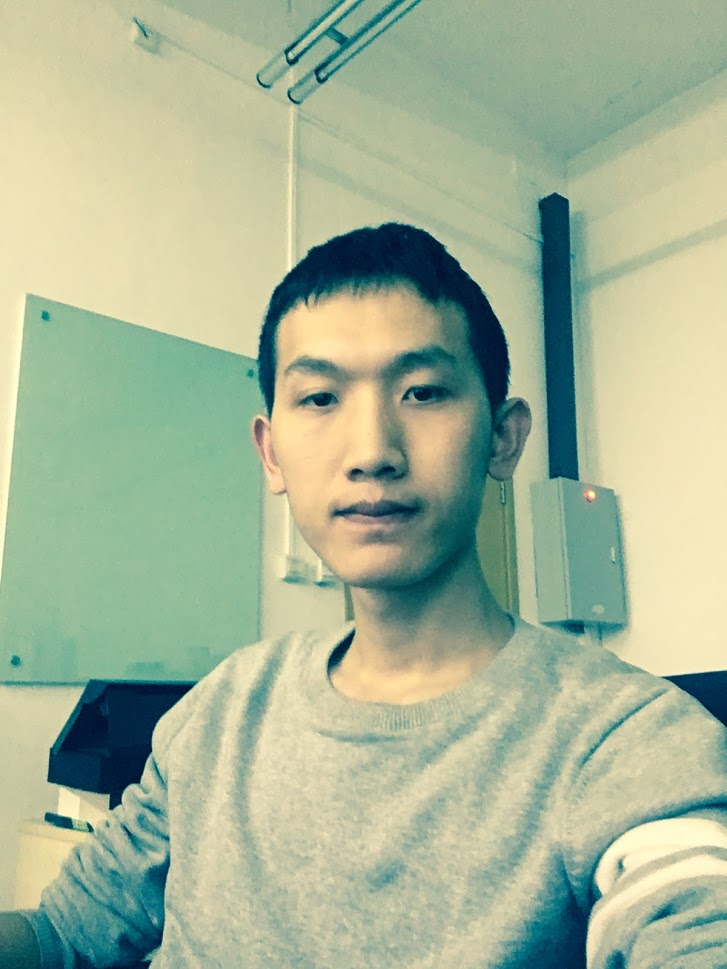
\includegraphics[width=4cm]{mathen}
\section{Contact}
~
13581724604
~
\section{Languages}
C++
Python
\section{Skills}
图形渲染OpenGL DX
图像处理OpenCV
\end{aside}

\begin{entrylist}

  \entry
    {2021.1-Now}
    {图形渲染算法工程师}
    {北京智源人工智能研究院}
    {
      \vspace{-5pt}
      \leftmargini=-1cm
      \begin{itemize}
        \setlength{\itemsep}{3pt}
        \item {基于OptiX的实时光线追踪的系统feature开发: tranparent, emissive 等}
        \item {GPU SDF实现和改进:构建GPU ConePillSDF来绘制复杂图形}
        \item {HDR和ToneMapping构建}
      \end{itemize}
      \vspace{5pt}
      \hspace{-1.2cm} \textbf{keywords:} \emph{RayTracing}, SDF
    }
  


  \entry
    {2018.7-2021.1}
    {图形学工程师-渲染引擎方向}
    {网易游戏}
    {
      \vspace{-5pt}
      \leftmargini=-1cm
      \begin{itemize}
        \setlength{\itemsep}{3pt}
        \item {TAA: 搭建引擎的TAA系统}
        \item {Cluster Shading: 实现高效的Forward+管线, 低带宽, 高cache命中率}
        \item {SAO: 实现高效的实用AO算法}
        \item {HiZ SSR: 实现HiZ以及使用HiZ的SSR}
        \item {性能优化: 指令优化, 数学拟合, cache和算法优化等}
        \item {算法创新:诸如描边算法的创新改进}
      \end{itemize}
      \vspace{5pt}
      \hspace{-1.2cm} \textbf{keywords:} \emph{Rendering}, HLSL, OpenGL, 移动端优化, C++, Python
    }
  
  \entry
    {2017.11-18.1}
    {实习生}
    {旷世科技}
    {
      \vspace{-5pt}
      \leftmargini=-1cm
      \begin{itemize}
        \setlength{\itemsep}{3pt}
        \item {人脸检测和ImageCaption调研}
      \end{itemize}
      \vspace{5pt}
      \hspace{-1.2cm} \textbf{keywords:} \emph{Facial recognition, C++}
    }
  
  \entry
    {2017.06-07}
    {实习生}
    {网易游戏}
    {
      \vspace{-5pt}
      \leftmargini=-1cm
      \begin{itemize}
        \setlength{\itemsep}{3pt}
        \item {保守光栅展UV}
        \item {设置图像质量衡量指标筛选质量不达标的贴图}
      \end{itemize}
      \vspace{5pt}
      \hspace{-1.2cm} \textbf{keywords:} OpenGL, OpenCV, 图像处理, C++, Python
    }
  
  \entry
    {2015.09 - 2018.07}
    {学生}
    {清华大学}
    {
      \vspace{-5pt}
      \leftmargini=-1cm
      \begin{itemize}
        \setlength{\itemsep}{3pt}
        \item {实现并比较多种图像融合算法:Multi-Splines,Modified Poisson,Convolution\\ Pyramid
        , Multi-Band,Mean-Value Coordinates等}
        \item {提出改进的卷积金字塔方法消除色彩渗透,生成效果更好的全景视频}
      \end{itemize}
      \vspace{5pt}
      \hspace{-1.2cm} \textbf{keywords:} \textbf{全景图像, 泊松方程, 调和插值, 频域卷积},{C++ , OpenCV}
  }
  
  \end{entrylist}



\section{Education}
\begin{entrylist}
\vspace{-10pt}
\entry
{2015 - 2018}
{图形学与计算几何实验室 {\normalfont ~~ 计算机专业~~清华大学}}
{ 硕士}
{}
\vspace{-10pt}
\entry
{2010 - 2014}
{计算机专业 {\normalfont ~~ 哈尔滨工业大学}}
{ 学士}
{ }
\end{entrylist}
\vspace{-5pt} 
\section{Publications}
\begin{entrylist}
\entry
{2018}
{A Comparative Study of Algorithms for Realtime Panoramic Video Blending.}
{TIP}
{ IEEE Trans. Image Processing 27(6): 2952-2965 (2018)}
\entry
{2017}
{Avoiding bleeding in image blending.}
{ICIP}
{IEEE International Conference on Image Processing}
\end{entrylist}
\vspace{-10pt}
\section{Awards}
\begin{entrylist}
  \vspace{5pt}
   \hspace{0.2cm}研究生期间的全景视频生成项目获得清华-腾讯联合实验室优秀项目奖\\
   \hspace{0.2cm}全景视频生成项目作为实验室项目的一部分参与了国家科技进步二等奖的申报并获奖
\end{entrylist}



%\end{aside}

\end{document}